\documentclass[a4paper]{article}

%% Language and font encodings
\usepackage[english]{babel}
\usepackage[utf8x]{inputenc}
\usepackage[T1]{fontenc}

%% Sets page size and margins
\usepackage[a4paper,top=3cm,bottom=2cm,left=3cm,right=3cm,marginparwidth=2cm]{geometry}

%% Useful packages
\usepackage{amsmath}
\usepackage{amsfonts}
\usepackage{bbm}
\usepackage{graphicx}
\usepackage[colorinlistoftodos]{todonotes}
\usepackage[colorlinks=true, allcolors=blue]{hyperref}
\usepackage{float}
\usepackage{enumerate}
\usepackage{mathrsfs}
\usepackage{subcaption}

\usepackage{tikz}
\tikzset{
    vertex/.style={circle,draw,minimum size=1.5em},
    edge/.style={->,> = latex'}
}

\title{Stochastic Processes}
\author{Kevin Chang}

\graphicspath{ {./images/} }

\begin{document}
\maketitle

\section{}
\begin{itemize}
\begin{figure} [H]
    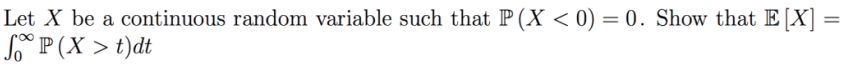
\includegraphics[width=1\linewidth]{question/1.png}
\end{figure}
    \item $\mathbb{E}[X]$
        $= \int_{-\infty}^\infty x f_X(x) dx$
        $= \int_0^\infty x f_X(x) dx$

        $= \int_0^\infty \int_0^x f_X(x) dt dx = \int_0^\infty \int_t^\infty f_X(x) dx dt = \int_0^\infty P[X > t] dt$
\end{itemize}

\section{}
\begin{itemize}
\begin{figure} [H]
    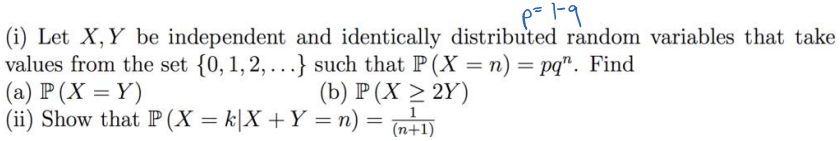
\includegraphics[width=1\linewidth]{question/2.png}
\end{figure}
    \item (i)
        \begin{itemize}
            \item (a)
                \begin{itemize}
                    \item $P[X=Y] = \sum_{n = 0}^\infty P[X=Y|X=n]P[X=n]$
                        $= \sum_{n = 0}^\infty P[Y=n|X=n]P[X=n]$
                        $= \sum_{n = 0}^\infty P[Y=n]P[X=n]$
                        $= \sum_{n = 0}^\infty p^2 \times q^{2n} = p^2 \frac{1}{1-q^2}$
                \end{itemize}
            \item (b)
                \begin{itemize}
                    \item $P[X\geq 2Y] = \sum_{n = 0}^\infty P[X\geq 2Y|Y=n]P[Y=n]$

                        $= \sum_{n = 0}^\infty P[X \geq 2n]P[Y=n]$
                        $= \sum_{n = 0}^\infty \frac{pq^{2n}}{1-q} pq^n$
                        $= \frac{p^2 q^{3n}}{(1-q)(1-q^3)}$
                \end{itemize}
        \end{itemize}
    \item (ii)
        \begin{itemize}
            \item $P[X=k|X+Y=n] = \frac{P[X=k, X+Y = n]}{P[X+Y=n]}$
                $= \frac{P[X=k, Y = n-k]}{\sum_{i=0}^nP[X=i] P[Y=n-i]}$

                $= \frac{pq^k \times pq^{n-k}}{\sum_{i=0}^n pq^i \times pq^{n-i}}$
                $= \frac{1}{(n+1)}$
        \end{itemize}
\end{itemize}

\section{}
\begin{itemize}
\begin{figure} [H]
    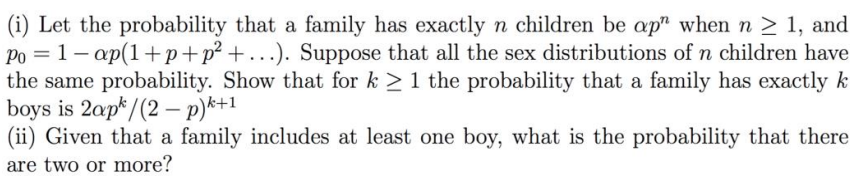
\includegraphics[width=1\linewidth]{question/3.png}
\end{figure}
    \item 
\end{itemize}

\section{}
\begin{itemize}
\begin{figure} [H]
    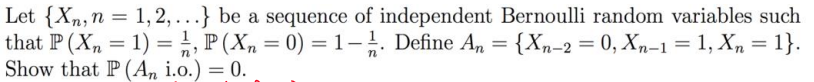
\includegraphics[width=1\linewidth]{question/4.png}
\end{figure}
    \item $P[A_n] = (1-\frac{1}{n-2})(\frac{1}{n-1})(\frac{1}{n}) = \frac{n-3}{(n-2)(n-1)n}$
    \item $\sum_{n = 1}^\infty P[A_n] < \infty \rightarrow P[A_n$ $f.o.] = 1$
    \item $P[A_n$ $i.o.] = 1 - P[A_n$ $f.o.] = 0$
\end{itemize}

\section{}
\begin{itemize}
\begin{figure} [H]
    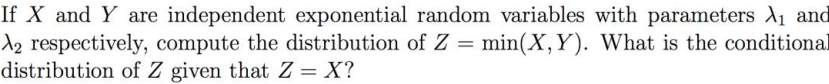
\includegraphics[width=1\linewidth]{question/5.png}
\end{figure}
    \item $P[Z \leq z]$
        \begin{itemize}
            \item $P[Z > z] = P[X > z, Y>z] = e^{-(\lambda_1 + \lambda_2)z}$
            \item $P[Z \leq z] = 1 - P[Z>z] = 1 - e^{-(\lambda_1 + \lambda_2)z}$
        \end{itemize}
    \item $P[Z \leq z | Z=X]$
        \begin{itemize}
            \item $P[Z > z | Z=X] = \frac{P[Y>X>z]}{P[Z=X]} = \frac{\int_z^\infty e^{-\lambda_2x} \lambda_1 e^{-\lambda_1x}dx}{\int_0^\infty e^{-\lambda_2x} \lambda_1 e^{-\lambda_1x}dx} = e^{-(\lambda_1 + \lambda_2)z}$
            \item $P[Z \leq z | Z=X] = 1 - P[Z>z | Z=X] = 1 - e^{-(\lambda_1 + \lambda_2)z}$
        \end{itemize}
\end{itemize}

\section{}
\begin{itemize}
\begin{figure} [H]
    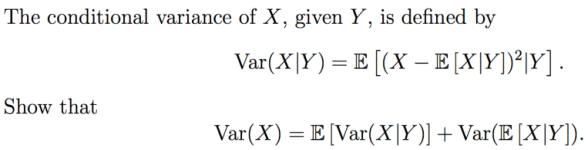
\includegraphics[width=0.7\linewidth]{question/6.png}
\end{figure}
    \item $\mathit{Var}(X|Y) = \mathbb{E}[(X-\mathbb{E}[X|Y])^2|Y]$
        $= \mathbb{E}[X^2 + \mathbb{E}[X|Y]^2 - 2X\mathbb{E}[X|Y]|Y]$

        $= \mathbb{E}[X^2|Y] + \mathbb{E}[\mathbb{E}[X|Y]^2|Y] - 2 \mathbb{E}[X|Y] \times \mathbb{E}[X|Y]$
        $= \mathbb{E}[X^2|Y] - \mathbb{E}[X|Y]^2$
    \item $\mathbb{E}[\mathit{Var}(X|Y)] = \mathbb{E}[\mathbb{E}[X^2|Y] - \mathbb{E}[X|Y]^2]$
        $= \mathbb{E}[X^2] - \mathbb{E}[\mathbb{E}[X|Y]^2]$
    \item $\mathit{Var}(\mathbb{E}[X|Y]) = \mathbb{E}[\mathbb{E}[X|Y]^2] - \mathbb{E}[\mathbb{E}[X|Y]]^2$
        $= \mathbb{E}[\mathbb{E}[X|Y]^2] - \mathbb{E}[X]^2$
    \item $\mathbb{E}[\mathit{Var}(X|Y)] + \mathit{Var}(\mathbb{E}[X|Y]) = \mathbb{E}[X^2] - \mathbb{E}[X]^2 = \mathit{Var}(X)$
\end{itemize}

\section{}
\begin{itemize}
\begin{figure} [H]
    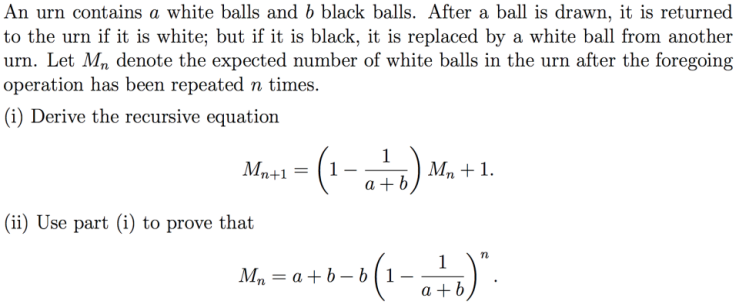
\includegraphics[width=1\linewidth]{question/7.png}
\end{figure}
    \item (i)
        \begin{itemize}
            \item Suppose the number of white balls in the urn after the $n$ times foregoing operation is $X_n$
            \item $P[X_{n+1} = k] = P[X_n = k] \frac{k}{a+b} + P[X_n = k-1] \frac{a+b-k+1}{a+b}$
            \item $\mathbb{E}[X_{n+1}] = \sum_{k=a}^{a+b} k P[X_{n+1}]$
                $= \sum_{k=a}^{a+b} k (P[X_n = k] \frac{k}{a+b} + P[X_n = k-1] \frac{a+b-k+1}{a+b})$

                $= \sum_{k=a}^{a+b} P[X_n = k] \frac{k^2}{a+b} + \sum_{k=a}^{a+b} P[X_n = k] (k+1) \frac{a+b-k}{a+b})$
                $= \sum_{k=a}^{a+b} P[X_n = k] (k - \frac{k}{a+b} + 1)$
                $= \mathbb{E}[X_n] (1-\frac{1}{a+b}) + 1$
            \item $M_{n+1} = (1-\frac{1}{a+b})M_n + 1$
        \end{itemize}
    \item (ii)
        \begin{itemize}
            \item $M_0 = a$ 
            \item $M_{n+1} = (1-\frac{1}{a+b})M_n + 1$
            \item $M_n = 1 + (1-\frac{1}{a+b}) + \dots + (1-\frac{1}{a+b})^{n-1} + a(1-\frac{1}{a+b})^n$
                $= \frac{(1-\frac{1}{a+b})^n - 1}{(1-\frac{1}{a+b}) - 1} + a(1-\frac{1}{a+b})^n$
                $= a + b - b(1-\frac{1}{a+b})^n$
        \end{itemize}
\end{itemize}

\section{}
\begin{itemize}
\begin{figure} [H]
    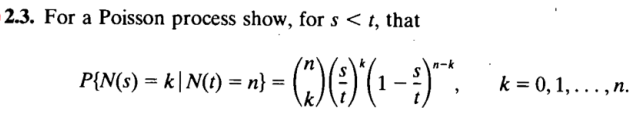
\includegraphics[width=0.6\linewidth]{question/8.png}
\end{figure}
    \item $P[N(s) = k| N(t) = n] = \frac{P[N(s) = k, N(t-s) = n-k]}{P[N(t) = n]}$
        $= \frac{\frac{(\lambda s)^k}{k!}e^{-\lambda s} \times \frac{(\lambda (t-s))^{n-k}}{(n-k)!}e^{-\lambda (t-s)}}{\frac{(\lambda t)^n}{n!}e^{-\lambda t}}$

        $= \binom{n}{k} (\frac{s}{t})^k (1 - \frac{s}{t})^{n-k}$
\end{itemize}

\end{document}
